% Drawing 154/09-4 -- folder 154, batch 09, archive page 166 (PDF page 167).
% Transcription: dessins en couleur sans texte : deux croquis de droites vert clair coupées de droites orange ; deux grands disques traversés de pseudo-droites rouges, secteurs coloriés en jaune, une partie du bord renforcée en vert foncé ou en noir, avec dans le premier une pseudo-droite en tirets noirs qui serpente et, au crayon, des hachures ; à droite, une bande horizontale faite de rectangles vert clair successifs, chacun traversé de droites rouges qui se croisent en losanges autour d'une ligne médiane noircie par segments
% Kind: lines cut by orange lines; two large disks with arrangements, yellow sectors, reinforced rims; band with cylinders. Method 2 (schematic redraw from the facsimile). Status: partial.
% Notes: Colour drawings without text over a job banner (16 Aug 82; not reproduced), read from the page view: two sketches of light green lines cut by orange lines; two large disks crossed by red-orange pseudolines, sectors coloured yellow (drawn as wedges), part of the rim reinforced in dark green or black, in the first a pencil sweep with a dashed black path, in the second small black bumps on the rim; at the bottom right a band of cylinders (light green verticals, red spindles and figure-eight strands, a dark middle line). Strands schematic.
% Coordinates: 1 unit = 1 mm = 1/100 of the crop width (bbox in page fractions: [0.207, 0.194, 0.964, 0.512]).
% Redrawn by Claude (claude-opus-5-5), issue #73, 2026-11-07; not checked by a human; not compiled (no TeX in the session).
% Rights: reproduces part of the work -- behind RENDER_TRANSCRIPTS, never published by itself.
\documentclass[tikz,border=3pt]{standalone}
\usepackage{amsmath,amssymb}
\usetikzlibrary{patterns,arrows.meta}
\tikzset{Or/.style={orange!90!black}, Ye/.style={yellow!80!orange}, Lg/.style={green!60!black!70}, Dg/.style={green!45!black}, Br/.style={brown!80!black}, Rd/.style={red!85!black}, Bl/.style={blue!70!black}, Gy/.style={black!40}, pencil/.style={black!45}, struck/.style={black!35}, mark/.style={circle,draw,inner sep=1.3pt}, pt/.style={circle,fill,inner sep=0.9pt}, opt/.style={circle,draw,fill=white,inner sep=1.1pt}}
\begin{document}
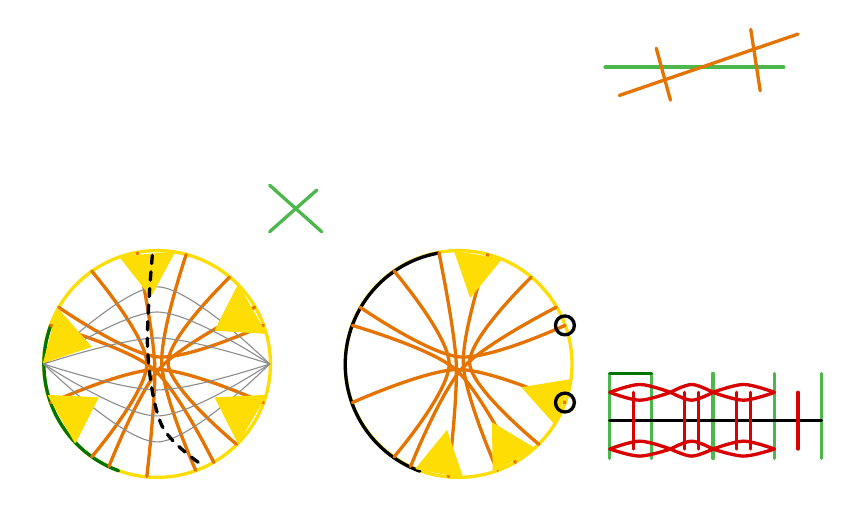
\begin{tikzpicture}[x=1mm,y=1mm,line cap=round,line join=round,font=\scriptsize]
\draw[Lg,very thick] (71.3,-6) -- (94,-6);
\draw[Or,very thick] (73.1,-9.6) -- (95.8,-1.8);
\draw[Or,very thick] (77.8,-3.6) -- (79.6,-10.2);
\draw[Or,very thick] (89.8,-1.2) -- (91,-9);
\draw[Lg,very thick] (28.7,-21) -- (35.3,-26.9);
\draw[Lg,very thick] (28.7,-26.9) -- (34.7,-21.6);
\draw[Ye,very thick] (14.4,-43.7) circle[radius=14.4];
\draw[Dg,very thick] (0.9,-38.8) arc[start angle=160, end angle=250, x radius=14.4, y radius=14.4];
\draw[Or,very thick] plot[smooth, tension=0.55] coordinates {(11.9,-29.6) (14.1,-43.7) (13.1,-58)};
\draw[Or,very thick] plot[smooth, tension=0.55] coordinates {(18.1,-29.8) (15,-43.7) (19.3,-57.2)};
\draw[Or,very thick] plot[smooth, tension=0.55] coordinates {(6.1,-31.9) (13.1,-43.7) (6.1,-55.5)};
\draw[Or,very thick] plot[smooth, tension=0.55] coordinates {(23.6,-32.7) (15.8,-43.6) (24.5,-53.9)};
\draw[Or,very thick] plot[smooth, tension=0.55] coordinates {(1.9,-36.5) (14.5,-42.8) (27.9,-38.8)};
\draw[Or,very thick] plot[smooth, tension=0.55] coordinates {(0.9,-48.6) (14.4,-44.4) (27.9,-48.6)};
\draw[Or,very thick] plot[smooth, tension=0.55] coordinates {(26.8,-36.5) (14.8,-44.2) (8.3,-56.7)};
\draw[Or,very thick] plot[smooth, tension=0.55] coordinates {(0.9,-38.8) (13.9,-44.3) (21.6,-56.2)};
\draw[pencil] plot[smooth, tension=0.55] coordinates {(0,-43.7) (14.4,-33.9) (28.7,-43.7)};
\draw[pencil] plot[smooth, tension=0.55] coordinates {(0,-43.7) (14.4,-37.1) (28.7,-43.7)};
\draw[pencil] plot[smooth, tension=0.55] coordinates {(0,-43.7) (14.4,-40.4) (28.7,-43.7)};
\draw[pencil] plot[smooth, tension=0.55] coordinates {(0,-43.7) (14.4,-47) (28.7,-43.7)};
\draw[pencil] plot[smooth, tension=0.55] coordinates {(0,-43.7) (14.4,-50.3) (28.7,-43.7)};
\draw[pencil] plot[smooth, tension=0.55] coordinates {(0,-43.7) (14.4,-53.6) (28.7,-43.7)};
\draw[Ye] (16.6,-29.5) -- (9.7,-30.1) -- (13.6,-35.1) -- cycle;
\fill[pattern=north east lines,Ye] (16.6,-29.5) -- (9.7,-30.1) -- (13.6,-35.1) -- cycle;
\draw[Ye] (1.8,-36.7) -- (0,-43.5) -- (6,-41.5) -- cycle;
\fill[pattern=north east lines,Ye] (1.8,-36.7) -- (0,-43.5) -- (6,-41.5) -- cycle;
\draw[Ye] (0.6,-47.7) -- (4,-53.7) -- (6.9,-48) -- cycle;
\fill[pattern=north east lines,Ye] (0.6,-47.7) -- (4,-53.7) -- (6.9,-48) -- cycle;
\draw[Ye] (24.7,-53.7) -- (28.2,-47.7) -- (21.8,-48) -- cycle;
\fill[pattern=north east lines,Ye] (24.7,-53.7) -- (28.2,-47.7) -- (21.8,-48) -- cycle;
\draw[Ye] (28.2,-39.8) -- (24.7,-33.7) -- (21.8,-39.4) -- cycle;
\fill[pattern=north east lines,Ye] (28.2,-39.8) -- (24.7,-33.7) -- (21.8,-39.4) -- cycle;
\draw[dashed,very thick] plot[smooth, tension=0.55] coordinates {(13.8,-29.9) (13.2,-41.9) (15,-51.5) (19.8,-56.3)};
\draw[Ye,very thick] (52.7,-43.7) circle[radius=14.4];
\draw[very thick] (50.2,-29.6) arc[start angle=100, end angle=250, x radius=14.4, y radius=14.4];
\draw[Or,very thick] plot[smooth, tension=0.55] coordinates {(50.2,-29.6) (52.4,-43.7) (51.4,-58)};
\draw[Or,very thick] plot[smooth, tension=0.55] coordinates {(56.4,-29.8) (53.3,-43.7) (57.6,-57.2)};
\draw[Or,very thick] plot[smooth, tension=0.55] coordinates {(44.5,-31.9) (51.5,-43.7) (44.5,-55.5)};
\draw[Or,very thick] plot[smooth, tension=0.55] coordinates {(61.9,-32.7) (54.1,-43.6) (62.9,-53.9)};
\draw[Or,very thick] plot[smooth, tension=0.55] coordinates {(40.2,-36.5) (52.8,-42.8) (66.2,-38.8)};
\draw[Or,very thick] plot[smooth, tension=0.55] coordinates {(39.2,-48.6) (52.7,-44.4) (66.2,-48.6)};
\draw[Or,very thick] plot[smooth, tension=0.55] coordinates {(65.1,-36.5) (53.2,-44.2) (46.6,-56.7)};
\draw[Or,very thick] plot[smooth, tension=0.55] coordinates {(39.2,-38.8) (52.2,-44.3) (59.9,-56.2)};
\draw[Ye] (58.1,-30.4) -- (52.2,-29.4) -- (54.2,-35.2) -- cycle;
\fill[pattern=north east lines,Ye] (58.1,-30.4) -- (52.2,-29.4) -- (54.2,-35.2) -- cycle;
\draw[Ye] (64.9,-51.3) -- (66.9,-45.7) -- (60.8,-46.7) -- cycle;
\fill[pattern=north east lines,Ye] (64.9,-51.3) -- (66.9,-45.7) -- (60.8,-46.7) -- cycle;
\draw[Ye] (57.1,-57.4) -- (62.3,-54.4) -- (57,-51.2) -- cycle;
\fill[pattern=north east lines,Ye] (57.1,-57.4) -- (62.3,-54.4) -- (57,-51.2) -- cycle;
\draw[Ye] (47.3,-57) -- (53.2,-58.1) -- (51.2,-52.2) -- cycle;
\fill[pattern=north east lines,Ye] (47.3,-57) -- (53.2,-58.1) -- (51.2,-52.2) -- cycle;
\draw[very thick] (66.2,-38.8) ellipse[x radius=1.2, y radius=1.2];
\draw[very thick] (66.2,-48.6) ellipse[x radius=1.2, y radius=1.2];
\draw[Lg,very thick] (71.9,-44.9) -- (71.9,-55.7);
\draw[Lg,very thick] (77.2,-44.9) -- (77.2,-55.7);
\draw[Lg,very thick] (85,-44.9) -- (85,-55.7);
\draw[Lg,very thick] (92.8,-44.9) -- (92.8,-55.7);
\draw[Lg,very thick] (98.8,-44.9) -- (98.8,-55.7);
\draw[very thick] (71.9,-50.9) -- (98.8,-50.9);
\draw[Dg,very thick] (71.9,-44.9) -- (77.2,-44.9);
\draw[Rd,very thick] plot[smooth, tension=0.55] coordinates {(71.9,-47.3) (75.7,-46.3) (79.6,-47.3)};
\draw[Rd,very thick] plot[smooth, tension=0.55] coordinates {(71.9,-47.3) (75.7,-48.3) (79.6,-47.3)};
\draw[Rd,very thick] plot[smooth, tension=0.55] coordinates {(71.9,-54.5) (75.7,-53.5) (79.6,-54.5)};
\draw[Rd,very thick] plot[smooth, tension=0.55] coordinates {(71.9,-54.5) (75.7,-55.4) (79.6,-54.5)};
\draw[Rd,very thick] plot[smooth, tension=0.55] coordinates {(79.6,-47.3) (82.3,-46.3) (85,-47.3)};
\draw[Rd,very thick] plot[smooth, tension=0.55] coordinates {(79.6,-47.3) (82.3,-48.3) (85,-47.3)};
\draw[Rd,very thick] plot[smooth, tension=0.55] coordinates {(79.6,-54.5) (82.3,-53.5) (85,-54.5)};
\draw[Rd,very thick] plot[smooth, tension=0.55] coordinates {(79.6,-54.5) (82.3,-55.4) (85,-54.5)};
\draw[Rd,very thick] plot[smooth, tension=0.55] coordinates {(85,-47.3) (88.9,-46.3) (92.8,-47.3)};
\draw[Rd,very thick] plot[smooth, tension=0.55] coordinates {(85,-47.3) (88.9,-48.3) (92.8,-47.3)};
\draw[Rd,very thick] plot[smooth, tension=0.55] coordinates {(85,-54.5) (88.9,-53.5) (92.8,-54.5)};
\draw[Rd,very thick] plot[smooth, tension=0.55] coordinates {(85,-54.5) (88.9,-55.4) (92.8,-54.5)};
\draw[Rd,very thick] (74.9,-47.3) -- (74.9,-54.5);
\draw[Rd,very thick] (81.4,-47.3) -- (81.4,-54.5);
\draw[Rd,very thick] (83.2,-47.3) -- (83.2,-54.5);
\draw[Rd,very thick] (88,-47.3) -- (88,-54.5);
\draw[Rd,very thick] (89.8,-47.3) -- (89.8,-54.5);
\draw[Rd,very thick] (95.8,-47.3) -- (95.8,-54.5);
\end{tikzpicture}
\end{document}
